\documentclass{article}

\usepackage{fancyhdr}
\usepackage{extramarks}
\usepackage{amsmath}
\usepackage{amsthm}
\usepackage{amsfonts}
\usepackage{empheq}
\usepackage{mathtools}
\usepackage{physics}
\usepackage{hyperref}
\usepackage[dvipsnames]{xcolor} 
\hypersetup{
	colorlinks,
	linkcolor=BrickRed,
}
\usepackage{tikz}
\usetikzlibrary {datavisualization.formats.functions}
\usepackage{graphicx}
\usepackage{subcaption}
\usepackage{neuralnetwork}
\usepackage{comment}


\newcommand\numberthis{\addtocounter{equation}{1}\tag{\theequation}}

%
% Basic Document Settings
%

\topmargin=-0.45in
\evensidemargin=0in
\oddsidemargin=0in
\textwidth=6.5in
\textheight=9.0in
\headsep=0.25in

\linespread{1.2}

\pagestyle{fancy}
\lhead{\hmwkAuthorName}
\chead{\hmwkClass: \hmwkTitle}
\rhead{\firstxmark}
\lfoot{\lastxmark}
\cfoot{\thepage}

\renewcommand\headrulewidth{0.4pt}
\renewcommand\footrulewidth{0.4pt}

\setlength\parindent{0pt}

%
% Create Question Sections
%

\newcommand{\enterQuestionHeader}[1]{
	\nobreak\extramarks{}{Question \arabic{#1} cont'd on next page\ldots}\nobreak{}
	\nobreak\extramarks{Question \arabic{#1} (cont'd)}{Question \arabic{#1} cont'd on next page\ldots}\nobreak{}
}

\newcommand{\exitQuestionHeader}[1]{
	\nobreak\extramarks{Question \arabic{#1} (cont'd)}{Question \arabic{#1} cont'd on next page\ldots}\nobreak{}
	\stepcounter{#1}
	\nobreak\extramarks{Question \arabic{#1}}{}\nobreak{}
}

\setcounter{secnumdepth}{0}
\newcounter{partCounter}
\newcounter{homeworkQuestionCounter}
\setcounter{homeworkQuestionCounter}{1}
\nobreak\extramarks{Question \arabic{homeworkQuestionCounter}}{}\nobreak{}

%
% Homework Question Environment
%
% This environment takes an optional argument. When given, it will adjust the
% problem counter. This is useful for when the problems given for your
% assignment aren't sequential. See the last 3 problems of this template for an
% example.
%
\newenvironment{homeworkQuestion}[1][-1]{
	\ifnum#1>0
	\setcounter{homeworkQuestionCounter}{#1}
	\fi
	\section{Question \arabic{homeworkQuestionCounter}}
	\rule{0.9\textwidth}{3pt}\\
	\setcounter{partCounter}{1}
	\enterQuestionHeader{homeworkQuestionCounter}
}{
	\exitQuestionHeader{homeworkQuestionCounter}
}

%
% Homework Details
%   - Title
%   - Due date
%   - Class
%   - Section/Time
%   - Instructor
%   - Author
%

\newcommand{\hmwkTitle}{HW\#6}
\newcommand{\hmwkDueDate}{}
\newcommand{\hmwkClass}{CpE 520}
\newcommand{\institute}{West Virginia University}
\newcommand{\hmwkClassInstructor}{Professor Nasser Nasrabadi}
\newcommand{\hmwkAuthorName}{\textbf{Ali Zafari}}

%
% Title Page
%

\title{
	\vspace{2in}
	\textmd{\textbf{\hmwkClass:\ \hmwkTitle}}\\
	\vspace{0.1in}\large{\institute}\\
%	\vspace{0.1in}\large{\textit{\hmwkClassInstructor}}
	\vspace{3in}
}

\author{\hmwkAuthorName}
\date{}

\renewcommand{\part}[1]{\textbf{\Large Part \Alph{partCounter}}\stepcounter{partCounter}\\}

\begin{document}
	
	\pagenumbering{gobble}% prevent cover page of numbering
	\maketitle
	\pagebreak % let cover page free to the end of page
	\pagenumbering{arabic} % start page numbering again from 1 and print them!
	\tableofcontents
	\pagebreak
	
	\begin{homeworkQuestion}
		
		\subsection{Part (a): Decision Boundaries}
		The neural network of question 1 is repeated in figure \ref{fig:q1_xor}. Nodes with indices equal to 0, have the value of 1 to generate the bias with their corresponding weights.
		
		\begin{figure}[h]
			\centering
			\begin{neuralnetwork}[height=5, nodespacing=1.5cm, layerspacing=3cm, nodesize=20pt]
				\newcommand{\nodetextclear}[2]{}
				\newcommand{\nodetextxnb}[2]{\ifnum #2=0 $\mathbf{X_0}$ \else\ifnum #2=1 $\mathbf{X_1}$ \else \ifnum #2=3 $\mathbf{X_2}$ \fi \fi \fi}
				\newcommand{\logiclabel}[1]{\,{$\scriptstyle#1$}\,}
				\newcommand{\nodetextH}[2]{\ifnum #2=0 $\mathbf{h_0}$ \else\ifnum #2=1 $\mathbf{h_1}$ \fi \fi}
				\newcommand{\nodetextY}[2]{$\mathbf{y}$}
				\newcommand{\linklabelsA}[4]{\logiclabel{+1}}
				\newcommand{\linklabelsBias}[4]{\ifnum#1=0 \logiclabel{-1.5} \else \logiclabel{-0.5} \fi}
				\newcommand{\linklabelsY}[4]{\logiclabel{-2}}
				\inputlayer[count=4, bias=true, text=\nodetextxnb, exclude={2, 4}]
				\hiddenlayer[count=2, bias=true, exclude={2}, , text=\nodetextH]
				\outputlayer[count=3, exclude={1, 3}, text=\nodetextY]
				\link[from layer=0, to layer=1, from node=0, to node=1, label=\linklabelsBias]
				\link[from layer=0, to layer=1, from node=1, to node=1, label=\linklabelsA]
				\link[from layer=0, to layer=1, from node=3, to node=1, label=\linklabelsA]
				\link[from layer=1, to layer=2, from node=1, to node=2, label=\linklabelsY]
				\link[from layer=1, to layer=2, from node=0, to node=2, label=\linklabelsBias]
				\link[from layer=0, to layer=2, from node=1, to node=2, label=\linklabelsA]
				\link[from layer=0, to layer=2, from node=3, to node=2, label=\linklabelsA]
			\end{neuralnetwork}
		\caption{XOR with only one node at hidden layer}
		\label{fig:q1_xor}
		\end{figure}
	To find the decision boundaries we are going to find the equations for the hidden layer and the output layer. We assumed Threshold Function as the activation function of every node.
	\begin{align*}
	\mathbf{h_1}&\mathbf{=\varphi(X_1+X_2-1.5)}\\
	\mathbf{y}&\mathbf{=\varphi(-2h_1+X_1+X_2-0.5)}
	\end{align*} 
	and the definition of Threshold function, $\varphi(x)$ is as follows:
	\begin{equation*}
	\varphi(x) = 
	\begin{cases}
		1 &\qquad\text{if}\quad x\geq0\\
		0 &\qquad\text{if}\quad x<0 \\
	\end{cases}
	\end{equation*}
	Decision boundary equation for hidden node could be obtained by putting the argument of its activation function equal to zero as:
	\begin{equation*}
	X_1+X_2-1.5 = 0
	\end{equation*}
	Decision boundary for node $\mathbf{h_1}$ is plotted in figure \ref{fig:q1_h1}. As it can be seen from that figure, this node does a Boolean AND operation on $\mathbf{X_1}$ and $\mathbf{X_2}$.
	
	\begin{figure}[h]
		\centering
		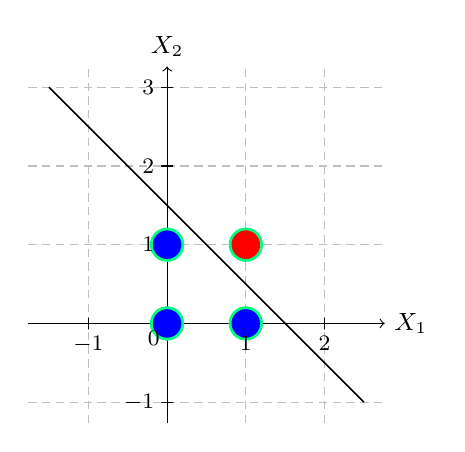
\begin{tikzpicture}
		\datavisualization [school book axes,
		all axes={grid},
		every grid/.append style={style=densely dashed},
		x axis={label=$X_1$},
		y axis={label=$X_2$},
		visualize as smooth line]
		data [format=function] {
			var x : interval [-1.5:2.5];
			func y = 1.5-\value x;
		}
		info {
			\filldraw [SpringGreen, fill=blue, line width=1pt] (visualization cs: x=0, y=0) circle [radius=2mm];
			\filldraw [SpringGreen, fill=blue, line width=1pt] (visualization cs: x=0, y=1) circle [radius=2mm];
			\filldraw [SpringGreen, fill=blue, line width=1pt] (visualization cs: x=1, y=0) circle [radius=2mm];
			\filldraw [SpringGreen, fill=red, line width=1pt] (visualization cs: x=1, y=1) circle [radius=2mm];
		};
		\end{tikzpicture}
		\caption{Node $\mathbf{h_1}$ decision boundary (AND operation)}
		\label{fig:q1_h1}
	\end{figure}
	
	Now we can discuss how the output node performs Boolean XOR with the aid of the only one hidden node. The decision boundary equation for output node is as follows:
	\begin{equation*}
	-2h_1+X_1+X_2-0.5 = 0
	\tag{*}
	\end{equation*}
	We know that the value of $\mathbf{h_1}$ is either one or zero depending on the inputs. Therefore we can imagine 2 ways of decision making for the output node.\\
	
	They are summarized below:\\\\
	\begin{tabular}{l  l c l}
		$\mathbf{h_1=0}$ (hidden node off)&$X_1+X_2-0.5 = 0$  &,&$\mathbf{X_1X_2} \in \{00, 01, 10\}$ \\\hline
		$\mathbf{h_1=1}$ (hidden node on)&$X_1+X_2-2.5 = 0$  &,&$\mathbf{X_1X_2=11}$
	\end{tabular}\\\\
	Now, we can plot the output node decision boundaries in two $\mathbf{X_1X_2}$ planes as it is in figure \ref{fig:q1_output}.

	\begin{figure}[h]
		\centering
		\begin{subfigure}{0.4\linewidth}
			\centering
			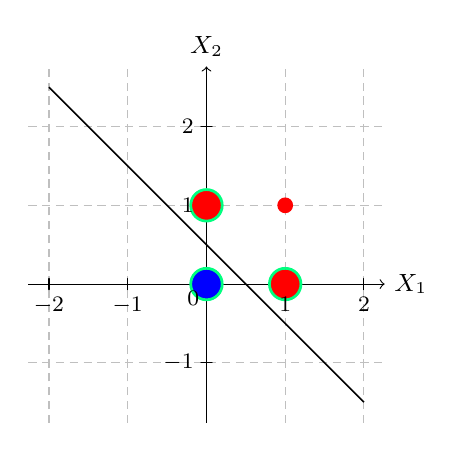
\begin{tikzpicture}
				\datavisualization [school book axes,
				all axes={grid},
				every grid/.append style={style=densely dashed},
				x axis={label=$X_1$},
				y axis={label=$X_2$},
				visualize as smooth line]
				data [format=function] {
					var x : interval [-2:2];
					func y = 0.5-\value x;
				}
				info {
					\filldraw [SpringGreen, fill=blue, line width=1pt] (visualization cs: x=0, y=0) circle [radius=2mm];
					\filldraw [SpringGreen, fill=red, line width=1pt] (visualization cs: x=0, y=1) circle [radius=2mm];
					\filldraw [SpringGreen, fill=red, line width=1pt] (visualization cs: x=1, y=0) circle [radius=2mm];
					\fill [red] (visualization cs: x=1, y=1) circle [radius=1mm];
				};
			\end{tikzpicture}
			\caption{when hidden node is off}
		\end{subfigure}
		\begin{subfigure}{0.4\linewidth}
			\centering
			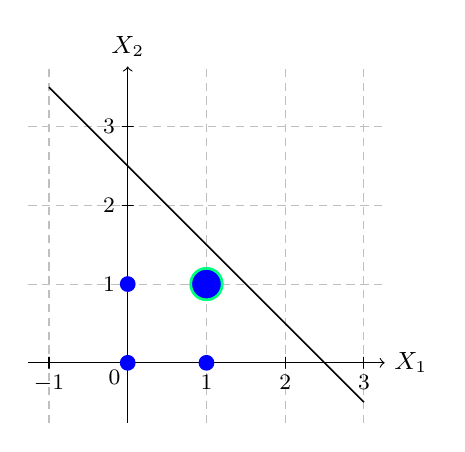
\begin{tikzpicture}
			\datavisualization [school book axes,
			all axes={grid},
			every grid/.append style={style=densely dashed},
			x axis={label=$X_1$},
			y axis={label=$X_2$},
			visualize as smooth line]
			data [format=function] {
				var x : interval [-1:3];
				func y = 2.5-\value x;
			}
			info {
				\fill [blue] (visualization cs: x=0, y=0) circle [radius=1mm];
				\fill [blue] (visualization cs: x=0, y=1) circle [radius=1mm];
				\fill [blue] (visualization cs: x=1, y=0) circle [radius=1mm];
				\filldraw [SpringGreen, fill=blue, line width=1pt]  (visualization cs: x=1, y=1) circle [radius=2mm];
			};
			\end{tikzpicture}
			\caption{when hidden node is on}
		\end{subfigure}
		\caption{Decision boundaries of output node ($\mathbf{y}$)}
		\label{fig:q1_output}
	\end{figure}
	\clearpage
	
	Another approach to view the decision boundary at the output node is to consider its hyperplane as a plane in 3D space, instead of a line in 2D space, as we did above. The plane of the equation $(*)$ in the 3d space of $X_1$, $X_2$ and $h_1$ is plotted in figure \ref{fig:q1_output_3d}. As it can be concluded form the truth table of the next section, the points $(0,1,0)$ and $(1,0,0)$ correspond to $X_1X_2=(0, 1)$ and $X_1X_2=(1, 0)$ respectively. Besides, the points $(0, 0, 0)$ and $(1, 1, 1)$ correspond to $X_1X_2=(0, 0)$ and $X_1X_2=(1, 1)$ respectively.
	
	\begin{figure}[tbh]
		\centering
		\begin{subfigure}{\columnwidth}
			\centering
			\includegraphics[width=\linewidth]{q1_3d_1}
		\end{subfigure}
		\begin{subfigure}{\columnwidth}
			\centering
			\includegraphics[width=\linewidth]{q1_3d_2}
		\end{subfigure}
		\caption{Decision boundary of output node ($\mathbf{y}$) in 3D space form 2 viewpoints }
		\label{fig:q1_output_3d}
	\end{figure}
	

		\clearpage
		\subsection{Part (b): Truth Table}	
		
		\begin{table}[h]
			\centering
			\caption{Truth Table}
				\begin{tabular}{c c|c|c}
					$\mathbf{X_1}$ & $\mathbf{X_2}$ & $\mathbf{h_1}$ & $\mathbf{y}$\\
					\hline\hline
					0 & 0 & 0 & 0\\\hline
					0 & 1 & 0 & 1\\\hline
					1 & 0 & 0 & 1\\\hline
					1 & 1 & 1 & 0
				\end{tabular}
					\label{tab:q1_truth}
		\end{table}

	\end{homeworkQuestion}
	\pagebreak
	
	\begin{homeworkQuestion}%Question 2
		\subsection{Part I}
		\subsubsection{(a): Decision Boundaries}
		The neural network of first part of question 2 is repeated in figure \ref{fig:q2_xor_1}. Nodes with indices equal to 0, have the value of 1 to generate the bias with their corresponding weights.
		\begin{figure}[h]
			\centering
			\begin{neuralnetwork}[height=5, nodespacing=2cm, layerspacing=5cm, nodesize=20pt]
				\newcommand{\nodetextclear}[2]{}
				\newcommand{\nodetextxnb}[2]{\ifnum #2=0 $\mathbf{X_0}$ \else\ifnum #2=1 $\mathbf{X_1}$ \else \ifnum #2=2 $\mathbf{X_2}$ \fi \fi \fi}
				\newcommand{\logiclabel}[1]{\,{$\scriptstyle#1$}\,}
				\newcommand{\nodetextH}[2]{\ifnum #2=0 $\mathbf{h_0}$ \else\ifnum #2=1 $\mathbf{h_1}$ \else \ifnum #2=2 $\mathbf{h_2}$ \fi \fi \fi}
				\newcommand{\nodetextY}[2]{$\mathbf{y}$}
				\newcommand{\linklabelsA}[4]{\logiclabel{+1}}
				\newcommand{\linklabelsBiasIn}[4]{\ifnum#4=1 \logiclabel{-0.5} \else \logiclabel{-1.5} \fi}
				\newcommand{\linklabelsBiasHidden}[4]{\logiclabel{-0.5}}
				\newcommand{\linklabelsY}[4]{\ifnum#2=1 \logiclabel{+1} \else \logiclabel{-1} \fi}
				\inputlayer[count=2, bias=true, text=\nodetextxnb]
				\hiddenlayer[count=2, bias=true, text=\nodetextH]
				\outputlayer[count=3, exclude={1, 3}, text=\nodetextY]
				\link[from layer=0, to layer=1, from node=0, to node=1, label=\linklabelsBiasIn, labelpos=very near start]
				\link[from layer=0, to layer=1, from node=0, to node=2, label=\linklabelsBiasIn, labelpos=very near start]
				\link[from layer=0, to layer=1, from node=1, to node=1, label=\linklabelsA, labelpos=very near start]
				\link[from layer=0, to layer=1, from node=2, to node=1, label=\linklabelsA, labelpos=very near start]
				\link[from layer=0, to layer=1, from node=1, to node=2, label=\linklabelsA, labelpos=very near start]
				\link[from layer=0, to layer=1, from node=2, to node=2, label=\linklabelsA, labelpos=very near start]
				\link[from layer=1, to layer=2, from node=0, to node=2, label=\linklabelsBiasHidden]
				\link[from layer=1, to layer=2, from node=1, to node=2, label=\linklabelsY]
				\link[from layer=1, to layer=2, from node=2, to node=2, label=\linklabelsY]
			\end{neuralnetwork}
			\caption{Neural network to check if it does Boolean XOR}
			\label{fig:q2_xor_1}
		\end{figure}
	To find the decision boundaries we are going to find the equations for the hidden layer and the output layer. We assumed Threshold Function as the activation function of every node.
	\begin{align*}
	\mathbf{h_1}&\mathbf{=\varphi(X_1+X_2-0.5)}\\
	\mathbf{h_2}&\mathbf{=\varphi(X_1+X_2-1.5)}\\
	\mathbf{y}&\mathbf{=\varphi(h_1-h_2-0.5)}
	\end{align*} 
	Decision boundaries for nodes $\mathbf{h_1}$ and $\mathbf{h_2}$ are plotted in figure \ref{fig:q2_hiddens_1}. As it can be seen from that figure, $\mathbf{h_1}$ does a Boolean OR operation on $\mathbf{X_1}$ and $\mathbf{X_2}$ and  $\mathbf{h_2}$ does AND on them.
	\begin{figure}[h]
		\centering
		\begin{subfigure}{0.4\linewidth}
			\centering
			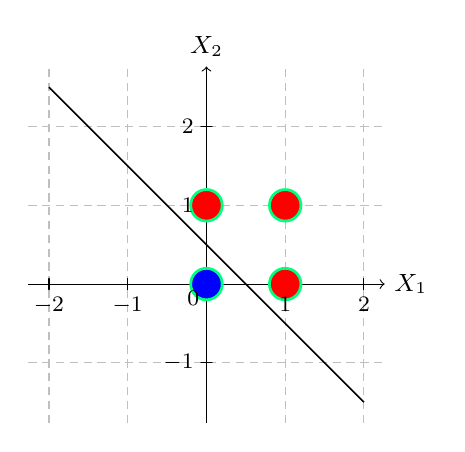
\begin{tikzpicture}
			\datavisualization [school book axes,
			all axes={grid},
			every grid/.append style={style=densely dashed},
			x axis={label=$X_1$},
			y axis={label=$X_2$},
			visualize as smooth line]
			data [format=function] {
				var x : interval [-2:2];
				func y = 0.5-\value x;
			}
			info {
				\filldraw [SpringGreen, fill=blue, line width=1pt] (visualization cs: x=0, y=0) circle [radius=2mm];
				\filldraw [SpringGreen, fill=red, line width=1pt] (visualization cs: x=0, y=1) circle [radius=2mm];
				\filldraw [SpringGreen, fill=red, line width=1pt] (visualization cs: x=1, y=0) circle [radius=2mm];
				\filldraw [SpringGreen, fill=red, line width=1pt] (visualization cs: x=1, y=1) circle [radius=2mm];
			};
			\end{tikzpicture}
			\caption{Node $\mathbf{h_1}$ decision boundary (OR)}
		\end{subfigure}
		\begin{subfigure}{0.4\linewidth}
			\centering
			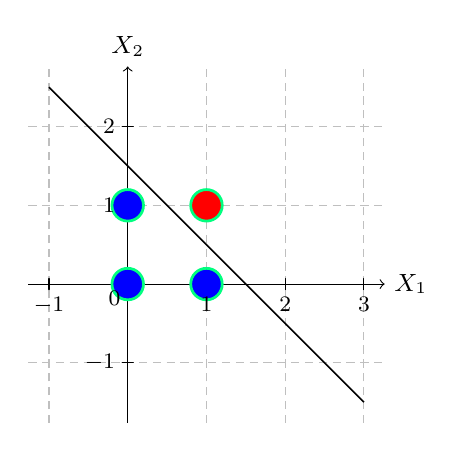
\begin{tikzpicture}
			\datavisualization [school book axes,
			all axes={grid},
			every grid/.append style={style=densely dashed},
			x axis={label=$X_1$},
			y axis={label=$X_2$},
			visualize as smooth line]
			data [format=function] {
				var x : interval [-1:3];
				func y = 1.5-\value x;
			}
			info {
				\filldraw [SpringGreen, fill=blue, line width=1pt]  (visualization cs: x=0, y=0) circle [radius=2mm];
				\filldraw [SpringGreen, fill=blue, line width=1pt]  (visualization cs: x=0, y=1) circle [radius=2mm];
				\filldraw [SpringGreen, fill=blue, line width=1pt]  (visualization cs: x=1, y=0) circle [radius=2mm];
				\filldraw [SpringGreen, fill=red, line width=1pt]  (visualization cs: x=1, y=1) circle [radius=2mm];
			};
			\end{tikzpicture}
			\caption{Node $\mathbf{h_2}$ decision boundary (AND)}
		\end{subfigure}
		\caption{ Decision boundaries of hidden layer}
		\label{fig:q2_hiddens_1}
	\end{figure}

		\begin{figure}[h]
			\centering
			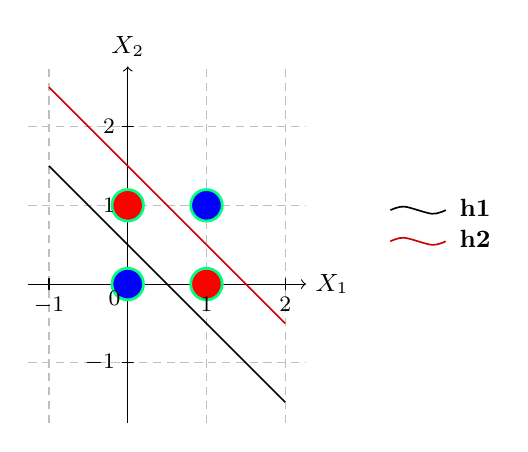
\begin{tikzpicture}
			\datavisualization [school book axes,
			all axes={grid},
			every grid/.append style={style=densely dashed},
			visualize as smooth line/.list={h1,h2},
			style sheet=strong colors,
			h1={label in legend={text=$\mathbf{h1}$}},
			h2={label in legend={text=$\mathbf{h2}$}},
			x axis={label=$X_1$},
			y axis={label=$X_2$},
			data/format=function,]
			data [set=h1] {
				var x : interval [-1:2];
				func y = 0.5-\value x;
			}
			data [set=h2] {
				var x : interval [-1:2];
				func y = 1.5-\value x;
			}
			info {
				\filldraw [SpringGreen, fill=blue, line width=1pt] (visualization cs: x=0, y=0) circle [radius=2mm];
				\filldraw [SpringGreen, fill=red, line width=1pt] (visualization cs: x=0, y=1) circle [radius=2mm];
				\filldraw [SpringGreen, fill=red, line width=1pt] (visualization cs: x=1, y=0) circle [radius=2mm];
				\filldraw [SpringGreen, fill=blue, line width=1pt] (visualization cs: x=1, y=1) circle [radius=2mm];
			};
		
			\end{tikzpicture}
			\caption{Output decision boundary}
			\label{fig:q2_output_1}
		\end{figure}
	
	We can also plot the decision boundary of the output node in the $h_1h_2$ plane. As it will be shown in the next section with the help of a truth table, the points $X_1X_2=(0, 1),(1, 0)$ are both mapped to the point $h_1h_2=(1, 0)$ and the hyperplane (line) of the output node could successfully discriminate them from the other two points to solve the XOR problem.
	
	\begin{figure}[h]
		\centering
		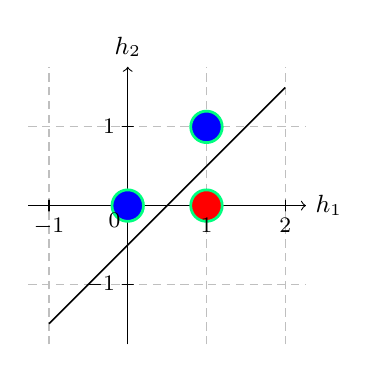
\begin{tikzpicture}
		\datavisualization [school book axes,
		all axes={grid},
		every grid/.append style={style=densely dashed},
		style sheet=strong colors,
		x axis={label=$h_1$},
		y axis={label=$h_2$},
		data/format=function,
		visualize as smooth line,]
		data{
			var x : interval [-1:2];
			func y = -0.5 + \value x) ;
		}
		info {
			\filldraw [SpringGreen, fill=blue, line width=1pt] (visualization cs: x=0, y=0) circle [radius=2mm];
			\filldraw [SpringGreen, fill=red, line width=1pt] (visualization cs: x=1, y=0) circle [radius=2mm];
			\filldraw [SpringGreen, fill=blue, line width=1pt] (visualization cs: x=1, y=1) circle [radius=2mm];
		};
		
		\end{tikzpicture}
		\caption{Output decision boundary ($h_1h_2$ plane)}
		\label{fig:q2_output_1_hplane}
	\end{figure}

	\subsubsection{(b): Truth Table}
	\begin{table}[h]
		\centering
		\caption{Truth Table}
		\begin{tabular}{c c|c|c|c}
			$\mathbf{X_1}$ & $\mathbf{X_2}$ & $\mathbf{h_1}$ & $\mathbf{h_2}$ & $\mathbf{y}$\\
			\hline\hline
			0 & 0 & 0 & 0 & 0\\\hline
			0 & 1 & 1 & 0 & 1\\\hline
			1 & 0 & 1 & 0 & 1\\\hline
			1 & 1 & 1 & 1 & 0
		\end{tabular}
		\label{tab:q2_truth_1}
	\end{table}
	As we have seen from the previous two sections, this neural network is capable of solving XOR problem.
	\pagebreak
	\subsection{Part II}
	\subsubsection{(a): Decision Boundaries}
	The neural network of second part of question 2 is repeated in figure \ref{fig:q2_xor_2}. Nodes with indices equal to 0, have the value of 1 to generate the bias with their corresponding weights.
	\begin{figure}[h]
		\centering
		\begin{neuralnetwork}[height=5, nodespacing=2cm, layerspacing=5cm, nodesize=20pt]
			\newcommand{\nodetextclear}[2]{}
			\newcommand{\nodetextxnb}[2]{\ifnum #2=0 $\mathbf{X_0}$ \else\ifnum #2=1 $\mathbf{X_1}$ \else \ifnum #2=2 $\mathbf{X_2}$ \fi \fi \fi}
			\newcommand{\logiclabel}[1]{\,{$\scriptstyle#1$}\,}
			\newcommand{\nodetextH}[2]{\ifnum #2=0 $\mathbf{h_0}$ \else\ifnum #2=1 $\mathbf{h_1}$ \else \ifnum #2=2 $\mathbf{h_2}$ \fi \fi \fi}
			\newcommand{\nodetextY}[2]{$\mathbf{y}$}
			\newcommand{\linklabelsAone}[4]{\ifnum#4=1 \logiclabel{-2} \else \logiclabel{+4.3} \fi}
			\newcommand{\linklabelsAtwo}[4]{\ifnum#4=1 \logiclabel{+9.2} \else \logiclabel{+8.8} \fi}
			\newcommand{\linklabelsBiasIn}[4]{\ifnum#4=1 \logiclabel{-1.8} \else \logiclabel{-0.1} \fi}
			\newcommand{\linklabelsBiasHidden}[4]{\logiclabel{-0.8}}
			\newcommand{\linklabelsY}[4]{\ifnum#2=1 \logiclabel{-4.5} \else \logiclabel{+5.3} \fi}
			\inputlayer[count=2, bias=true, text=\nodetextxnb]
			\hiddenlayer[count=2, bias=true, text=\nodetextH]
			\outputlayer[count=3, exclude={1, 3}, text=\nodetextY]
			\link[from layer=0, to layer=1, from node=0, to node=1, label=\linklabelsBiasIn, labelpos=very near start]
			\link[from layer=0, to layer=1, from node=0, to node=2, label=\linklabelsBiasIn, labelpos=very near start]
			\link[from layer=0, to layer=1, from node=1, to node=1, label=\linklabelsAone, labelpos=very near start]
			\link[from layer=0, to layer=1, from node=2, to node=1, label=\linklabelsAtwo, labelpos=very near start]
			\link[from layer=0, to layer=1, from node=1, to node=2, label=\linklabelsAone, labelpos=very near start]
			\link[from layer=0, to layer=1, from node=2, to node=2, label=\linklabelsAtwo, labelpos=very near start]
			\link[from layer=1, to layer=2, from node=0, to node=2, label=\linklabelsBiasHidden]
			\link[from layer=1, to layer=2, from node=1, to node=2, label=\linklabelsY]
			\link[from layer=1, to layer=2, from node=2, to node=2, label=\linklabelsY]
		\end{neuralnetwork}
		\caption{Neural network to check if it does Boolean XOR}
		\label{fig:q2_xor_2}
	\end{figure}
		To find the decision boundaries we are going to find the equations for the hidden layer and the output layer. We assumed Threshold Function as the activation function of every node.
		\begin{align*}
		\mathbf{h_1}&\mathbf{=\varphi(-2X_1+9.2X_2-1.8)}\\
		\mathbf{h_2}&\mathbf{=\varphi(4.3X_1+8.8X_2-0.1)}\\
		\mathbf{y}&\mathbf{=\varphi(-4.5h_1+5.3h_2-0.8)}
		\end{align*}
		Decision boundaries for nodes $\mathbf{h_1}$ and $\mathbf{h_2}$ are plotted in figure \ref{fig:q2_hiddens_2}. As it can be seen from that figure, $\mathbf{h_2}$ does a Boolean OR operation on $\mathbf{X_1}$ and $\mathbf{X_2}$ but $\mathbf{h_1}$'s classification is not a known Boolean operation.\\
		
		\begin{figure}[h]
			\centering
			\begin{subfigure}{0.4\linewidth}
				\centering
				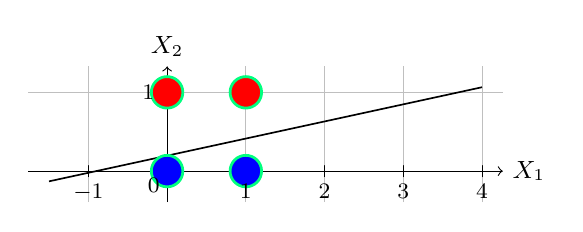
\begin{tikzpicture}
				\datavisualization [school book axes,
				all axes={grid},
				x axis={label=$X_1$},
				y axis={label=$X_2$},
				visualize as smooth line]
				data [format=function] {
					var x : interval [-1.5:4];
					func y = (1.8/9.2)+((2/9.2)*\value x) ;
				}
				info {
					\filldraw [SpringGreen, fill=blue, line width=1pt] (visualization cs: x=0, y=0) circle [radius=2mm];
					\filldraw [SpringGreen, fill=red, line width=1pt] (visualization cs: x=0, y=1) circle [radius=2mm];
					\filldraw [SpringGreen, fill=blue, line width=1pt] (visualization cs: x=1, y=0) circle [radius=2mm];
					\filldraw [SpringGreen, fill=red, line width=1pt] (visualization cs: x=1, y=1) circle [radius=2mm];
				};
				\end{tikzpicture}
				\caption{Node $\mathbf{h_1}$ decision boundary}
			\end{subfigure}
			\begin{subfigure}{0.4\linewidth}
				\centering
				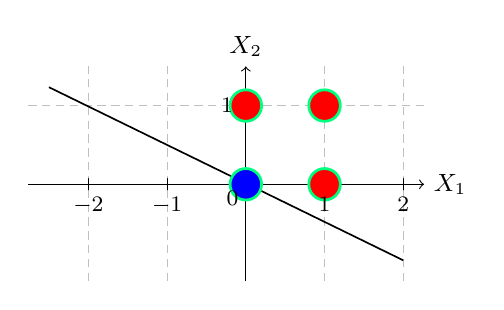
\begin{tikzpicture}
				\datavisualization [school book axes,
				all axes={grid},
				every grid/.append style={style=densely dashed},
				x axis={label=$X_1$},
				y axis={label=$X_2$},
				visualize as smooth line]
				data [format=function] {
					var x : interval [-2.5:2];
					func y = (0.1/8.8)+((-4.3/8.8)*\value x) ;
				}
				info {
					\filldraw [SpringGreen, fill=blue, line width=1pt]  (visualization cs: x=0, y=0) circle [radius=2mm];
					\filldraw [SpringGreen, fill=red, line width=1pt]  (visualization cs: x=0, y=1) circle [radius=2mm];
					\filldraw [SpringGreen, fill=red, line width=1pt]  (visualization cs: x=1, y=0) circle [radius=2mm];
					\filldraw [SpringGreen, fill=red, line width=1pt]  (visualization cs: x=1, y=1) circle [radius=2mm];
				};
				\end{tikzpicture}
				\caption{Node $\mathbf{h_2}$ decision boundary (OR)}
				\label{fig:q2_hiddens_2_b}
			\end{subfigure}
			\caption{ Decision boundaries of hidden layer}
			\label{fig:q2_hiddens_2}
		\end{figure}
	
	(the line in figure \ref{fig:q2_hiddens_2_b} goes slightly above the point (0, 0))
	
	\pagebreak
	Now we can plot decision boundary of the output node in the $h_1h_2$ plane. As it will be shown in the next section with the help of a truth table, the points $X_1X_2=(0, 1),(1, 1)$ are both mapped to the point $h_1h_2=(1, 1)$ and the hyperplane (line) of the output node will pass exactly through this point, so they will both get the same label and apparently this is not correct for an XOR problem.
	\begin{figure}[h]
		\centering
		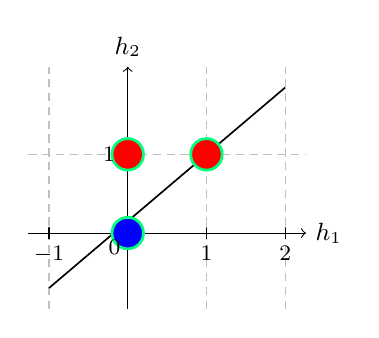
\begin{tikzpicture}
		\datavisualization [school book axes,
		all axes={grid},
		every grid/.append style={style=densely dashed},
		style sheet=strong colors,
		x axis={label=$h_1$},
		y axis={label=$h_2$},
		data/format=function,
		visualize as smooth line,]
		data{
			var x : interval [-1:2];
			func y = (0.8/5.3)+((4.5/5.3)*\value x) ;
		}
		info {
			\filldraw [SpringGreen, fill=blue, line width=1pt] (visualization cs: x=0, y=0) circle [radius=2mm];
			\filldraw [SpringGreen, fill=red, line width=1pt] (visualization cs: x=0, y=1) circle [radius=2mm];
			\filldraw [SpringGreen, fill=red, line width=1pt] (visualization cs: x=1, y=1) circle [radius=2mm];
		};
		
		\end{tikzpicture}
		\caption{Output decision boundary ($h_1h_2$ plane)}
		\label{fig:q2_output_2}
	\end{figure}
	
		\subsubsection{(b): Truth Table}
		For the inputs $X_1X_2 \in \{01, 11\}$ input argument of the $\varphi$ will be exactly zero, so it depends on which value we have defined for the $\varphi(0)$. Therefore, by any definition, this neural network will not solve the XOR problem correctly.
		\begin{table}[h]
			\centering
			\caption{Truth Table}
			\begin{tabular}{c c|c|c|c}
				$\mathbf{X_1}$ & $\mathbf{X_2}$ & $\mathbf{h_1}$ & $\mathbf{h_2}$ & $\mathbf{y}$\\
				\hline\hline
				0 & 0 & 0 & 0 & 0\\\hline
				0 & 1 & 1 & 1 & 1 (or 0)?\\\hline
				1 & 0 & 0 & 1 & 1\\\hline
				1 & 1 & 1 & 1 & 1 (or 0)?
			\end{tabular}
			\label{tab:q2_truth_2}
		\end{table}
	\end{homeworkQuestion}

	
\end{document}